\section{Mechanism of the break}
\label{sec:mechanism}

\Cref{sec:precursor,sec:buffer} are direct inspections of raw training
curves; \cref{sec:earlyinit} uses the per-episode action-amplitude log
(\cref{sec:gsac,sec:setup}). \Cref{fig:mechanism} summarizes the two
surviving mechanistic results.

\subsection{The break is sudden and precursor-free}
\label{sec:precursor}

For all four algorithms, in every seed with a mid-training break (seeds 0, 1,
3, 4), the mean and standard deviation of the reward are stable over the
40-episode window immediately before the break --- no ramp, no gradual
degradation (\cref{tab:prebreak}). The longest-runway confirmations come from
$\text{seed}=4$, where \texttt{sac\_high} (break at 131) and
\texttt{gsac\_high} (break at 122) each have a full 40-episode pre-break
window flat to within noise: $-32.29\!\to\!-32.32$ (s.d.\ 1.09) and
$-32.29\!\to\!-32.08$ (s.d.\ 1.18) respectively (\cref{fig:mechanism}a).

\begin{table}[t]
\centering
\caption{Pre-break reward statistics (40-episode window where the runway
allows, else the full pre-break run; seed $=0\,/\,1\,/\,4$).}
\label{tab:prebreak}
\small
\begin{tabular}{|l|c|c|c|}
\hline
Algorithm & First-half mean & Second-half mean & Std.\ dev. \\
\hline
PPO  & $-32.75\,/\,{-32.28}\,/\,{-32.36}$ & $-32.77\,/\,{-33.05}\,/\,{-32.39}$ & $1.35\,/\,1.32\,/\,0.91$ \\
\hline
SAC  & $-33.31\,/\,{-32.76}\,/\,{-32.29}$ & $-32.50\,/\,{-32.79}\,/\,{-32.32}$ & $1.30\,/\,1.39\,/\,1.09$ \\
\hline
GPPO & $-32.61\,/\,{-32.38}\,/\,{-32.60}$ & $-32.98\,/\,{-33.01}\,/\,{-33.05}$ & $1.10\,/\,1.24\,/\,1.34$ \\
\hline
GSAC & $-32.49\,/\,{-32.19}\,/\,{-32.29}$ & $-32.46\,/\,{-32.08}\,/\,{-32.08}$ & $1.32\,/\,1.16\,/\,1.18$ \\
\hline
\end{tabular}
\end{table}

GPPO/GSAC analytic-gradient norms over the 15 episodes before the break are
similarly flat (\cref{fig:gradnorm}). The break is therefore not the policy
\emph{gradually} driving the solver past its limit, but a sudden, stochastic
event --- a single episode's randomly sampled action sequence, combined with
the current policy, pushing the flow past the solver's $\Re\approx 350$--$380$
numerical-stability limit (\cref{sec:env}) --- consistent with the
butterfly-effect trigger expected from Metz et al.~\cite{metz2021} and the
Re-shrunk predictability horizon of Boffetta and Musacchio~\cite{boffetta2017}.

\subsection{On-policy vs.\ off-policy after the trigger: buffer dilution}
\label{sec:buffer}

In on-policy PPO/GPPO the trigger episode's rollout is used in that same
episode's update, so trigger and permanent collapse always coincide --- no
escape, in any of the 10 on-policy runs (\cref{tab:trigger}). Off-policy
training \emph{could} in principle dilute the poisoned transitions in its
replay buffer. Whether it does depends on how full the buffer is at the
trigger. Let a run trigger at episode $e$, so the buffer holds $\approx 15e$
transitions of which $\approx 15$ are poisoned; the probability that
\emph{none} of the $10\times 64 = 640$ sampled transitions across the 10
post-trigger updates is poisoned is
\begin{equation}
  P_{\text{survive}}(e)\;\approx\;\left(1-\frac{15}{15\,e}\right)^{640}
  \;=\;\left(1-\frac{1}{e}\right)^{640}.
  \label{eq:survive}
\end{equation}
\Cref{eq:survive} is negligible unless $e\gtrsim 120$ (\cref{fig:mechanism}b):
a run triggering at episode 36 has $P_{\text{survive}}\approx 0$, whereas one
triggering at episode 141 has $P_{\text{survive}}\approx 1\%$. Only GSAC
triggers late enough (seeds 0 and 4, episodes 141 and 122) for this to be
non-negligible.

\begin{table}[t]
\centering
\caption{Trigger episode vs.\ recovery. ``Recovered'' $=$ intermediate
episodes with a valid (non-NaN) reward between trigger and permanent
collapse. Across all 20 $\Re=300$ runs exactly one shows a recovery window:
$\text{seed}=0$ GSAC (2 episodes).}
\label{tab:trigger}
\small
\begin{tabular}{|l|c|c|}
\hline
Algorithm & Trigger (s0\,/\,s1\,/\,s2\,/\,s3\,/\,s4) & Recovered \\
\hline
PPO  & $12\,/\,35\,/\,117\,/\,14\,/\,11$   & $0\,/\,0\,/\,0\,/\,0\,/\,0$ \\
\hline
SAC  & $36\,/\,6\,/\,2\,/\,40\,/\,131$     & $0\,/\,0\,/\,0\,/\,0\,/\,0$ \\
\hline
GPPO & $83\,/\,40\,/\,32\,/\,6\,/\,16$     & $0\,/\,0\,/\,0\,/\,0\,/\,0$ \\
\hline
GSAC & $141\,/\,63\,/\,2\,/\,45\,/\,122$   & $\mathbf{2}\,/\,0\,/\,0\,/\,0\,/\,0$ \\
\hline
\end{tabular}
\end{table}

\Cref{fig:mechanism}b plots \cref{eq:survive} against the actual trigger
episodes of the ten off-policy runs in \cref{tab:trigger}, with the single
observed recovery window circled.

\begin{figure}[t]
\centering
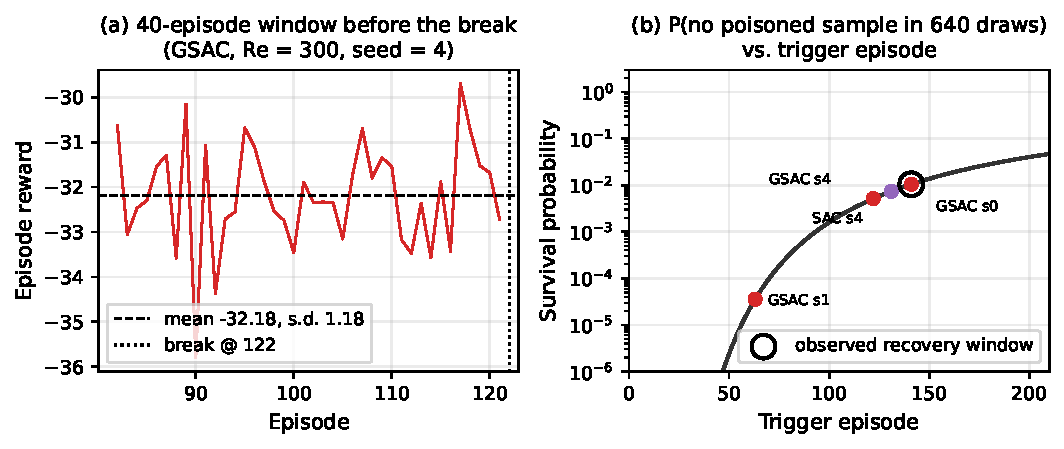
\includegraphics[width=\linewidth]{fig_mechanism.pdf}
\caption{Two surviving mechanistic results. (a) The 40-episode reward window
before the break (GSAC, $\Re=300$, $\text{seed}=4$): flat to within noise,
then an abrupt divergence. (b) The buffer-dilution survival probability of
\cref{eq:survive} vs.\ trigger episode; markers are the actual off-policy
runs, and the single observed recovery window (circled, $\text{seed}=0$
GSAC, trigger 141) is the one case where $P_{\text{survive}}$ is $\sim$1\%.}
\label{fig:mechanism}
\end{figure}

\Cref{eq:survive} gives a non-zero survival
probability only for a GSAC run that triggers past $\sim$episode 120. Two of
the five GSAC runs meet this ($\text{seed}=0$ at 141, $\text{seed}=4$ at 122);
the model predicts a recovery window is \emph{possible but rare} ($\sim$1\%)
for these and effectively impossible for the other 18 runs. Observed: one
window, in $\text{seed}=0$ GSAC. This is consistent with the model, but with
one positive across 20 runs the mechanism is suggestive, not
confirmed; a controlled buffer-size sweep at a fixed trigger is needed to
establish the $\sim$1\% rate.

\subsection{Divergence before learning: the early-init failure mode}
\label{sec:earlyinit}

The $\text{seed}=2$ sweep exposes a second, qualitatively different failure
mode. In $\text{seed}=2$ at $\Re=300$, both SAC and GSAC break at
episode 2 with an \emph{identical} episode-1 trajectory: same reward
($-33.68$), same action RMS ($0.308$), same action abs-max ($0.489$). This
identity is expected --- SAC and GSAC share the seed's initialization and
diverge only after episode 1, when GSAC applies its extra analytic step ---
yet both reach NaN on episode 2.

The logs rule out the \cref{sec:buffer} mechanism and an action-explosion
mechanism alike. GSAC's episode-1 analytic-gradient norm is 54,
squarely in the normal range ($\text{seed}=0$: 49, $\text{seed}=1$: 69 over
their first ten episodes), so the analytic step was not anomalous; and the
episode-2 rollout's action RMS is 0.307 with abs-max 0.485,
indistinguishable from episode 1, so the policy is not driving the flow with
large control.
What remains is that $\text{seed}=2$'s randomly initialized policy, composed
with the $\Re=300$ base flow, integrates to numerical divergence within two
episodes --- before any actor-learning algorithm has a foothold. Bare SAC
diverges identically, so this is a property of where the random
initialization lands relative to the solver's stability boundary
(\cref{sec:env}), not of analytic-gradient injection. GSAC's long runways in
seeds 0, 1, 4 (141, 63, 122 episodes) require several non-diverged episodes
for the analytic gradient to accumulate a stabilizing effect; $\text{seed}=2$
provides no such runway.

This mode is rare: 1 of 5 seeds. Seeds 3 and 4 both break
mid-training, so the episode-2 collapse is not the typical $\Re=300$
behaviour --- it is a low-probability tail of the same sudden,
precursor-free, stochastic trigger of \cref{sec:precursor}, occurring at
episode 2 instead of 45--141. It still reframes GSAC as highest
ceiling, no reliable floor, and shows the trigger-episode distribution
reaches all the way down to episode 2.

\Cref{sec:buffer} is a plausibility calculation
for the post-trigger lock-in; \cref{sec:earlyinit} shows \emph{when} the
trigger can occur. Neither explains \emph{why} a given (seed, init) triggers
at a given episode. The action-amplitude log now in place is the instrument
for this; a dedicated short-horizon re-run of seeds 0--1 logging the per-step
action norm is the next diagnostic (\cref{sec:conclusion}).
